\documentclass[conference]{assets/latex/IEEEtran}

\usepackage{amsmath,amssymb,amsfonts}
\usepackage{graphicx}
\usepackage{textcomp}
\usepackage{xcolor}
\usepackage[backend=biber,style=numeric]{biblatex}
\addbibresource{assets/latex/report.bib}

\graphicspath{{assets/latex/}}

\begin{document}

\title{CS6524 Computer Vision Lab. 2\\ Camera Calibration and Stereo Vision}

\author{\IEEEauthorblockN{Dara Heaphy}
\IEEEauthorblockA{\textit{Student ID 23369914} \\
University of Limerick\\
Limerick, Ireland \\
23369914@studentmail.ul.ie}
}

\maketitle

\begin{abstract}
I calibrated my phone camera and then used two frames of the same video as a
stereo pair to measure depth in cm. Calibration got to 0.37\,px RMS. With the
board at 62\,cm my depth was off by about 9\,cm, and at 115\,cm by about
25\,cm, mostly because the camera only moves a few cm between frames.
\end{abstract}

% =====================================================================
\section{Introduction}
We were asked to get real depth from a single handheld camera. If you take two
frames from a video a moment apart, they work like a stereo pair, but you
don't know how far the camera moved or how it turned. So I had to calibrate
the camera, work out how it moved between frames, and then run stereo
matching. For each scene I output a depth video in cm and a point cloud.

% =====================================================================
\section{Methodology}

\subsection{Data}
I filmed everything on an iPhone (1080$\times$1920, 30\,fps) and shrink every
frame to 360$\times$640 first, which keeps the whole run to about 25\,s. The
brief says the board has a 9$\times$6 inner grid, but mine has 9$\times$6
squares, so only 8$\times$5 inner corners. Nothing was detected until I
spotted this. The squares are 25\,mm. In scene 01 the board is about 60\,cm
away with a notebook and a box in front; in scene 02 it's about 115\,cm away.

\subsection{Calibration}
I look for the board in every second frame, split the video into 25 chunks,
and keep the sharpest frame from each, so I get a spread of angles without
blurry or repeated frames. I refine the corners with \texttt{cornerSubPix} and
run \texttt{calibrateCamera}.

It took three tries. In the first I didn't tilt the board enough (1.73\,px
error). In the second the paper bent while I moved it (1.97\,px). I knew it
was bending because the focal length jumped between 751 and 1159\,px
depending on which frames I used. For the third I taped the sheet to
something rigid, which gave Table~\ref{tab:calib}. The numbers look right: the
two focal lengths are almost equal, and the centre point is close to the
middle of the image.

\begin{table}[t]
\caption{Camera parameters at 360$\times$640}
\centering
\begin{tabular}{@{}llll@{}}
\hline
$f_x$ & 418.77 px & $k_1$ & $-0.0296$ \\
$f_y$ & 417.21 px & $k_2$ & $-0.0999$ \\
$c_x$ & 179.07 px & $k_3$ & $\phantom{-}0.0938$ \\
$c_y$ & 312.94 px & $p_1$ & $-0.0090$ \\
skew & 0 & $p_2$ & $-0.0023$ \\
\hline
\multicolumn{4}{@{}l}{Reprojection error: RMS 0.366 px, mean 0.283 px} \\
\hline
\end{tabular}
\label{tab:calib}
\end{table}

\begin{figure}[t]
\centerline{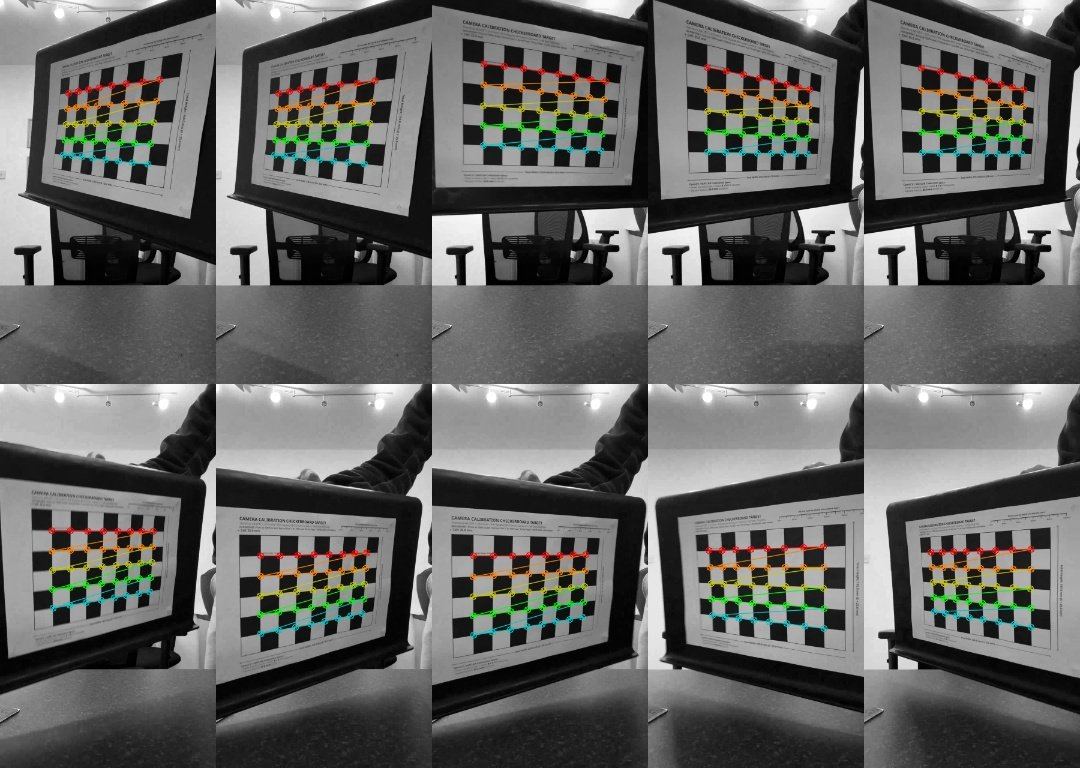
\includegraphics[width=\columnwidth]{corners.jpg}}
\caption{Some of my calibration frames with the detected corners.}
\label{fig:corners}
\end{figure}

\subsection{Camera motion between frames}
I match SIFT features between two frames, keeping only clear matches (ratio
test, 0.75). From the matches I estimate the essential matrix and get the
camera's rotation and direction of movement from it with
\texttt{recoverPose}.

At first I used back-to-back frames, but the camera barely moves between them
(under 2\,px), and only about 1\% of matches agreed. Using frames 20 apart
fixed this. I also tried getting the fundamental matrix first and converting
it, but that was 15--19$^\circ$ off compared to 12$^\circ$ for finding the
essential matrix directly. I think that's because the essential matrix already
uses the calibration. In scene 01 every one of the 123 pairs worked, with a
median direction error of 3.8$^\circ$, and in scene 02 120 of 126 did.

\subsection{Scale and depth}
The problem is that this only tells you which way the camera moved, not how
far. To get the distance I used the checkerboard: \texttt{solvePnP} gives the
camera's position in cm in every frame, I smooth that path, and the distance
between two frames is the baseline. Having the board close matters: the
position wobbled by 1.2\,cm with the board at 115\,cm but only 0.1\,cm at
60\,cm, so I re-filmed scene 01 with it closer. The baselines ended up at
roughly 2--4\,cm (scene 01) and 3--7\,cm (scene 02).

I then rectify the pair (line the two images up so matches are on the same
row), run SGBM to get the disparity, and turn that into depth using the focal
length and baseline. When the disparity is tiny, a 1\,px mistake changes the
depth a lot (about 30\% at 3\,px), so I drop anything below 3\,px. I use a log
colour scale in cm, because the scenes go from about 15\,cm to several metres
and on a normal scale everything close up was one colour.

\subsection{Point cloud (bonus)}
I take the frame with the best board accuracy and turn every pixel into a 3D
point, up to 4\,m away. At object edges SGBM mixes up foreground and
background, which gives stray points floating in between, so I drop pixels
whose depth jumps a lot compared to their neighbours, plus any isolated
points. The clouds have about 104k and 136k points.

% =====================================================================
\section{Results}
To check the depth I compare it with the board, since I know exactly where
the board is from \texttt{solvePnP} (Table~\ref{tab:depth}). About 60--70\% of
pixels get a depth. In Fig.~\ref{fig:depth} the objects in front, the board
and the wall come out in the right order, and the gaps are on plain walls and
far-away areas. In CloudCompare the point cloud (Fig.~\ref{fig:cloud}) looks
like the room, just patchy where the depth is missing.

\begin{table}[t]
\caption{Depth error at the checkerboard (median)}
\centering
\begin{tabular}{@{}lcccc@{}}
\hline
Scene, motion from & True depth & Baseline & Bias & Error \\
\hline
01, SIFT  & 62 cm  & 3.2 cm & $+2.1$ cm  & 9.1 cm \\
01, board & 62 cm  & 3.2 cm & $-0.4$ cm  & 3.9 cm \\
02, SIFT  & 115 cm & 5.8 cm & $+20.1$ cm & 24.6 cm \\
02, board & 115 cm & 5.8 cm & ---        & 53.5 cm \\
\hline
\end{tabular}
\label{tab:depth}
\end{table}

\begin{figure}[t]
\centerline{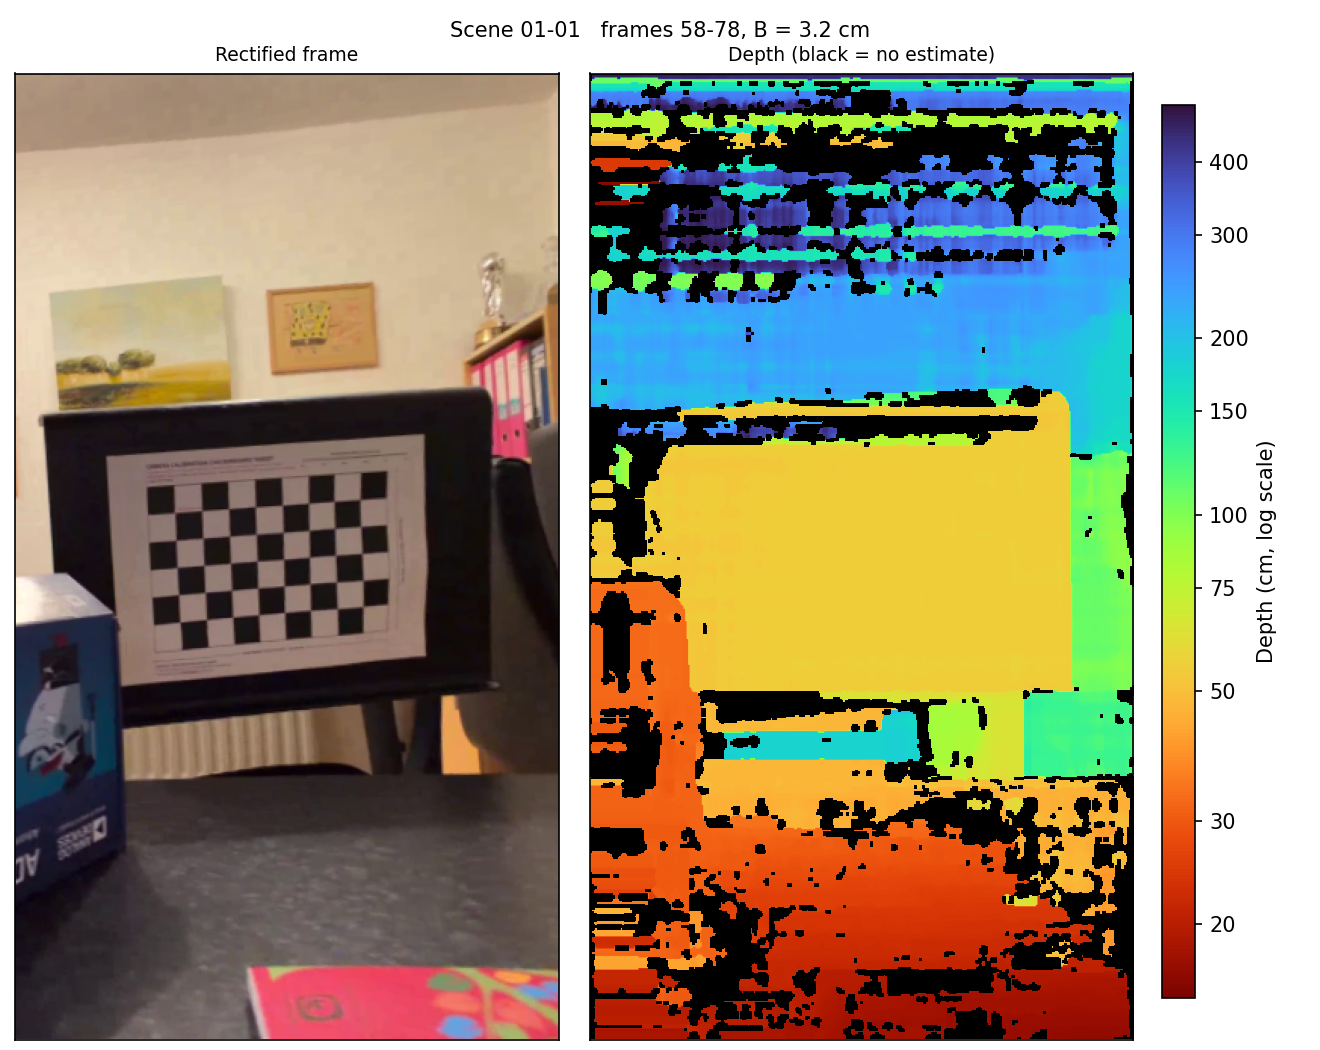
\includegraphics[width=\columnwidth]{depth_0101.png}}
\caption{Scene 01: image and depth in cm. Black means no depth.}
\label{fig:depth}
\end{figure}

\begin{figure}[t]
\centerline{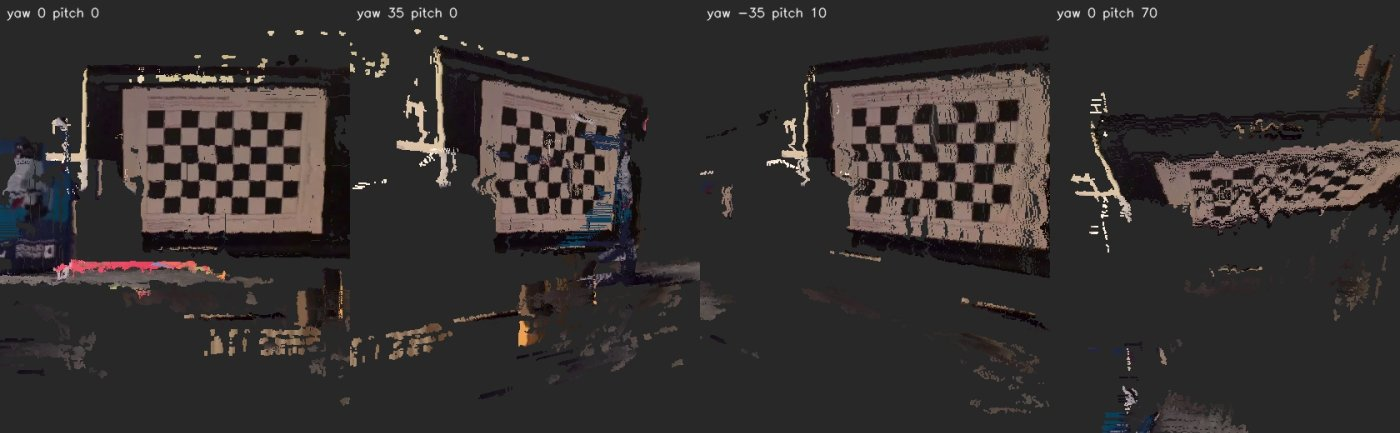
\includegraphics[width=\columnwidth]{cloud_0101.jpg}}
\caption{Scene 01 point cloud from four angles.}
\label{fig:cloud}
\end{figure}

% =====================================================================
\section{Discussion and Failure Analysis}
\textbf{Calibration.} It works, but only once the board was flat. Most of my
early error came from the board, not the code. Steeply tilted frames still
have more error (0.4--0.6\,px vs 0.1--0.2\,px), probably because the corners
are squashed and blurrier.

\textbf{Distance.} Scene 02 is worse mainly because the board is twice as far
away. Depth error grows quickly with distance, so the same small matching
mistake costs a lot more there. Moving a phone by hand only gives a few cm of
baseline, so anything past about 4.5\,m gets cut off.

\textbf{Camera motion.} Up close, the SIFT motion estimate is the weak point.
Using the board's motion instead cut scene 01's error from 9.1 to 3.9\,cm,
because a few degrees off means the two images aren't lined up properly. But
at 115\,cm the board itself is too wobbly and the error went up to 53.5\,cm.
The checkerboard also confuses SIFT, since all the squares look the same, and
plain walls give no matches at all, which leaves holes.

\textbf{What I'd do next.} Pick the frame gap based on how much the camera
actually moved, refine the motion over many frames at once (bundle
adjustment), combine depth from several pairs to fill holes, work at a higher
resolution, use a bigger board kept close, and film a more different second
scene, like outdoors.

% =====================================================================
\section{Conclusion}
The pipeline gets depth in cm from one moving phone, to within about 15\% at
60\,cm. The biggest things I learned were to keep the calibration board flat,
and that the small baseline and the motion estimate are what limit the depth.

\nocite{foundationsCVbook}
\printbibliography

\end{document}
